% Chapter Template

\chapter{Introduction} % Main chapter title

\label{Chapter1} % Change X to a consecutive number; for referencing this chapter elsewhere, use \ref{ChapterX}

%----------------------------------------------------------------------------------------
%	SECTION 1
%----------------------------------------------------------------------------------------
Taking a photograph of an object, traditionally, we need to face a camara (detector) to the object. But with two-photon imaging 
we use a detector that is towards the light source, rather than towards the object.
As the name suggest it, we also use the information about another photon that is strongly correlated. (IMAGE)
 Two-photon is reproduced at quantum level by a non-factorizable point-to-point image-forming correlation between two photons.

Two-photon imaging has been demonstrated using two types of light sources. Type-one
two-photon imaging uses entangled photon pairs as the light source. In 1995 Pittman, realized a 
quantum two-photon geometric optical effect.  They have successfully performed optical 
imaging by means of a quantum-mechanical entangled source\cite{pittman}.

Type-two of imaging uses chaotic light. The type-two  
image-forming correlation is caused by the superposition between paired two-photon amplitudes,
or the symmetrized effective two-photon wave-function\cite{physicsGhost}.
\section{Imaging}

Assuming we have an object that have its own light or its externally illuminated,
imaging means collecting that light that is emitted from the object. Each point
of the surface od the object will emit spherical waves to all possible directions,
been this said, What is the probability to have a spherical wave collapsing into a point or small spot? 
Obviously, the chance is practically zero unless an imaging system is applied.
\\
The concept of optical imaging was well developed in classical optics and the Figure
\ref{fig:imaging} schematically illustrates a standar imaging setup. In this setup 
an object is illuminated by a radiation source, an imaging lens is used 
to focus the scattered and reflected light from the object onto an image plane 
which is defined by the “Gaussian thin lens equation”\cite{hecht}:
\begin{equation}
\frac{1}{s_0}+\frac{1}{s_i}=\frac{1}{f}
\end{equation}
 where $s_0$ is the distance between the object and the imaging lens, $s_i$ the distance 
between the imaging lens and the image plane, and $f$ the focal lenght of the imaging lens. This equation defines
a point-to-point relationship between the object plane and the image plane: any radiation starting from a point on the object will colapse at a certain point at the image plane.
\\
\begin{figure}[h!]
\centering
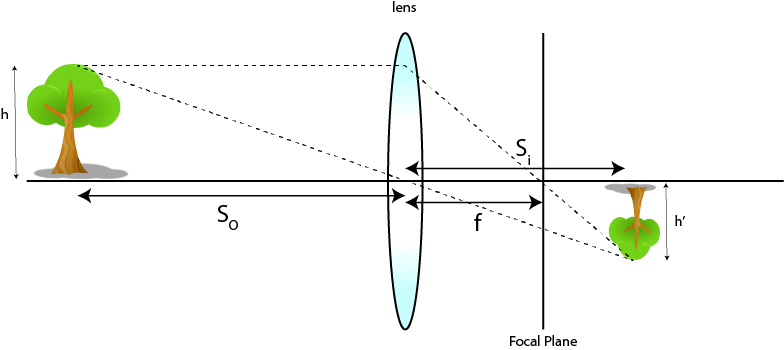
\includegraphics[width=0.6\textwidth]{Figures/imaging.png}
\caption{Optical imaging: a lens produces an image on an object at $f+d$. This distance is defined
by the Gaussian thin-lens equation $\frac{1}{l}+\frac{1}{f+d}=\frac{1}{f}$} 
\label{fig:imaging}
\end{figure}
This one-to-one correspondence in the image-forming relationship between the object and the image planes produces a perfect image.
The observed image can be magnified or demagnified, for example, in the 
Figure \ref{fig:imaging} the original object is a tree, and it is demagnified at the image plane. This depends on which optical 
system are we using, what kind on lenses are involved and the distance between object and them.


%-----------------------------------
%	SUBSECTION 1
%-----------------------------------
\section{Two-Photon Imaging}
Two-photon imaging consist after all, in reconstructing an image of an object. But in this case we use two dectector located in diferents paths of the light. By using the dectections of them separately we get a constant signal, with no information about the object, Figure \ref{fig:twoPhotonSetup}. But if instead we use the signal of them both, counting conincidences, we can reconstruct the double slit in Figure \ref{fig:twoPhotonSetup}. \\


\begin{figure}[h]
\centering
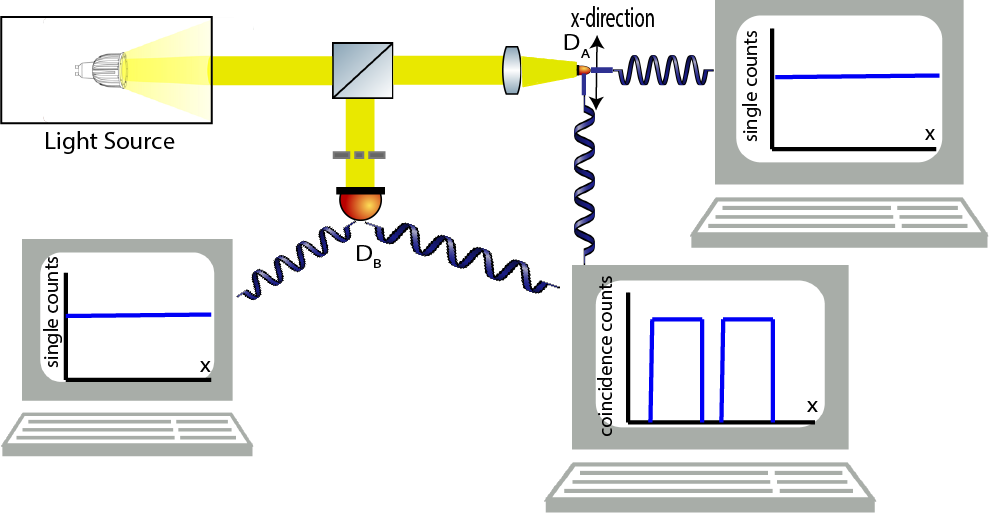
\includegraphics[width=0.7\textwidth]{Figures/twoPhotonSetup.png}
\caption{Simple schematic for the Two-photon Imaging} 
\label{fig:twoPhotonSetup}
\end{figure}
In order to reconstruct the image of the double slit, we have to introduce some kind of spatial dependence, the object, in this case the double slit, is distributed along a transverse direction of the light propagation. But what we have learnt is that scanning along the x-direction (asuming that light propagates along the z-direction), in the path that have no interaction with the object $D_2$, and colecting all the light that interacts with the object $D_1$, gathering no spatial information. We reconstruct the double slit in the coincidences counts, every time we have a photon detected going througt the double slit, and a photon at a certaint position $x_i$, we graph coincidences vs ${ x_i }$ and we get the image of the double slit, Figure \ref{fig:twoPhotonSetup}. 

\subsection{Two-Photon Imaging using entangled photon pairs}

In the previous section we introduced the notion of two-photon imaging , but we didn't care much about the nature of the source light. For this case we will use entangled photon as the source light, we will separate the pair of entangled photons by means of a polarization beamspliter. The first type-one two-photon imaging experiment was demonstrated by Pittman in 1995\cite{pittman}. The schematic setup of the experiment is shown in the Figure \ref{fig:pittman}. \\ 

\begin{figure}[h]
\centering
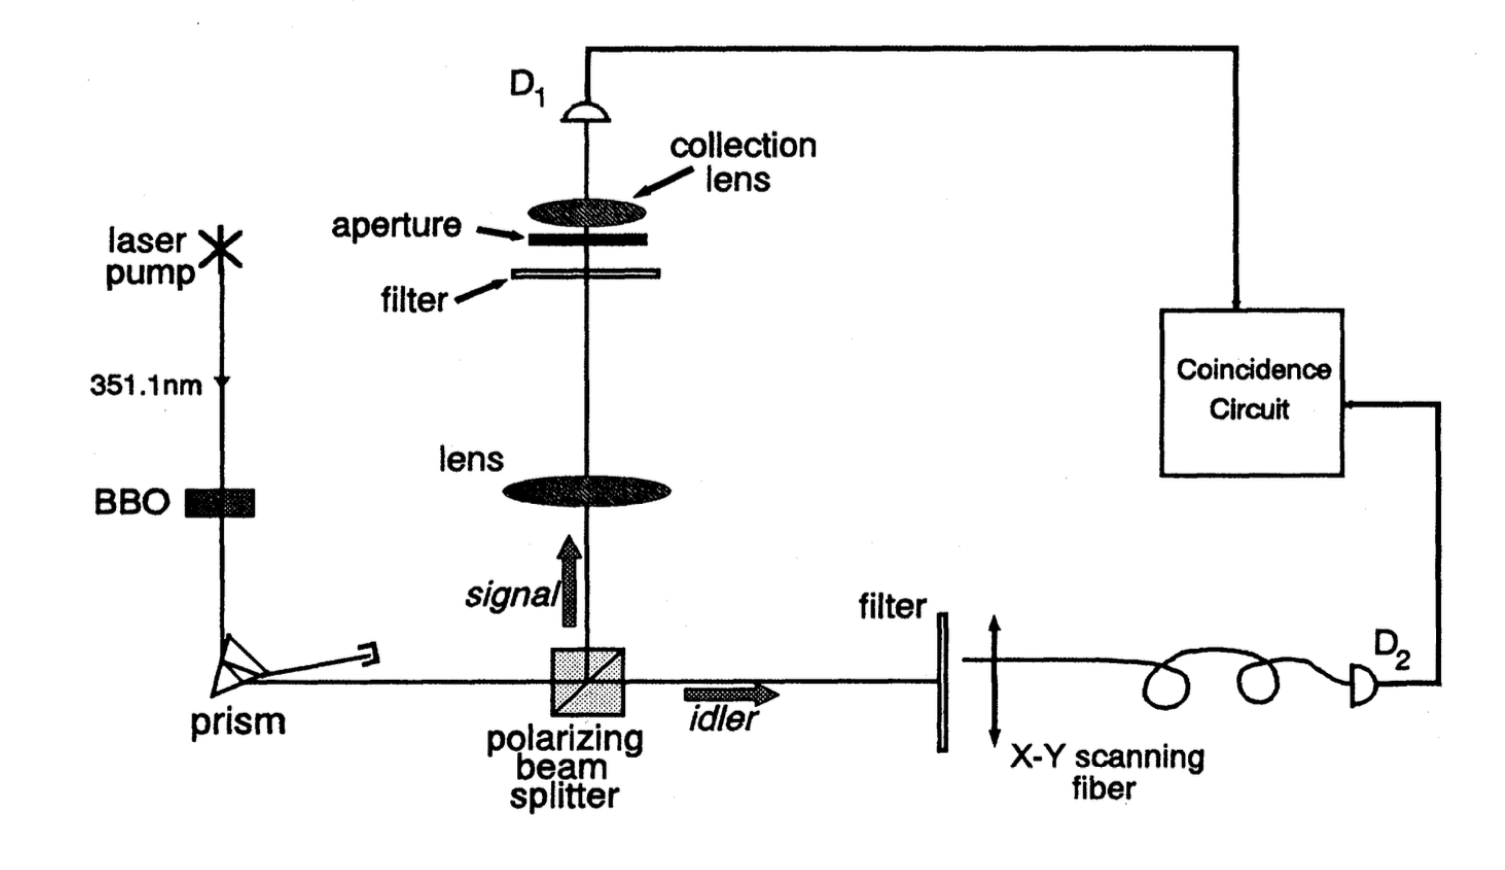
\includegraphics[width=0.5\textwidth]{Figures/pittman.png}
\caption{Schematic of the first "two-photon imaging" experimental setup, used by Pittman\cite{pittman}} 
\label{fig:pittman}
\end{figure}
A continuous wave (CW) laser is used to pump a nonlinear 
crystal to produce pairs of entangled photons. This pairs of orthogonally polarized signal and idler photons are the product
of the nonlinear optical process of spontaneous parametric down-conversion (SPDC).
The pair emerges from the crystal collinearly\footnote{The pairs emerge from the crystal nearly 
collinearly, with $\omega_s \simeq \omega_i \simeq \omega_p / 2$. where the subscript
letter stands for signal, idler and pump respectively}, it is separated by a dispersion prism, 
and then the signal and idler are sent in different directions by a polarization
beam slitting Glan-Thompson prism. 

The reflected signal beam passes through a 
convex lens with a $400mm$ focal length and illuminates an aperture\footnote{The aperture 
consisted of the letters UMBC, University of Maryland Baltimore County.}.
Before the aperture is placed a filter (Figure \ref{fig:signal}), 
this is a bandwidth spectral filters centered at the
wavelength $702.2 nm$. 
Behind the aperture is the detector package $D_1$. \\
\begin{figure}[H]
\centering
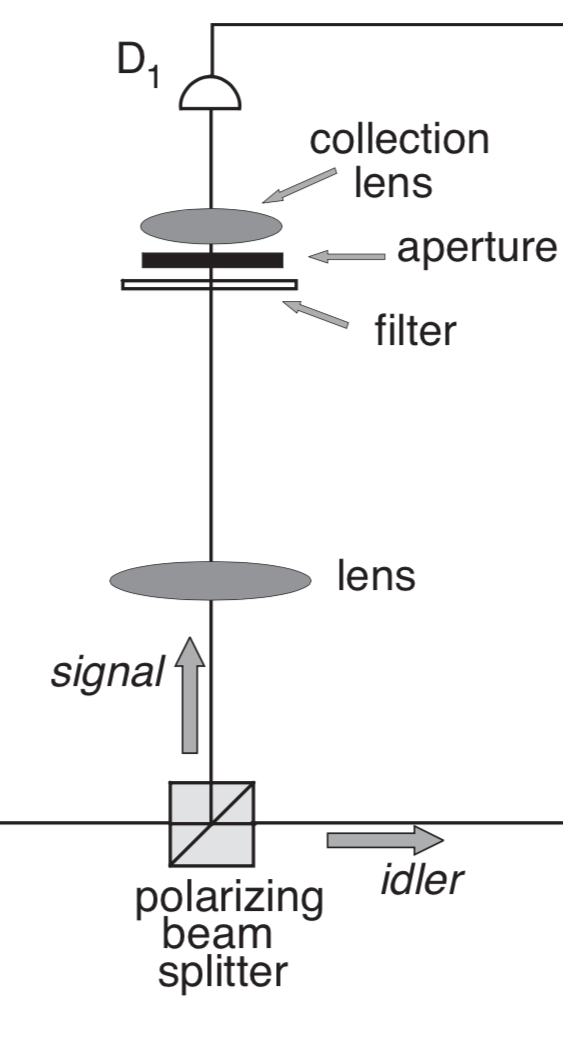
\includegraphics[width=0.24\textwidth]{Figures/signal.png}
\caption{The reflected photon, called signal} 
\label{fig:signal}
\end{figure}


The transmitted idler beam is met by detector 
package $D_2$. The input tip of the fiber is scanned in the transverse 
plane. The counts are sent to a coincidence 
counting circuit with a $1.8ns$ acceptance window.


An important fact of this experiment is the use of a lens(collection lens) in the signal beam that establishes an image plane with the definitive point-by-point correspondence object(mask) plane.




\subsection{Two-photon Imaging Using Thermal Sources}

In principle the term "thermal radiation" should refer only to radiation coming 
from a blackbody in thermal equilibrium at some temperature T. But with this realisation of thermal radiation
we have to face some characteristics of true thermal fields. Thermal radiation is also referred as chaotic light, which
have extreme short coherence time.  \textit{expand coherence time}

Thermal sources have to be understood as incoherent light, this means that we have many photons at the beam, but the frequencies they have are 
randonly distributed. In the case of entangled light, we had a light source that generated photons that all are around a given frequency, we used a diode laser at $405nm$.


\begin{figure}[h!]
\centering
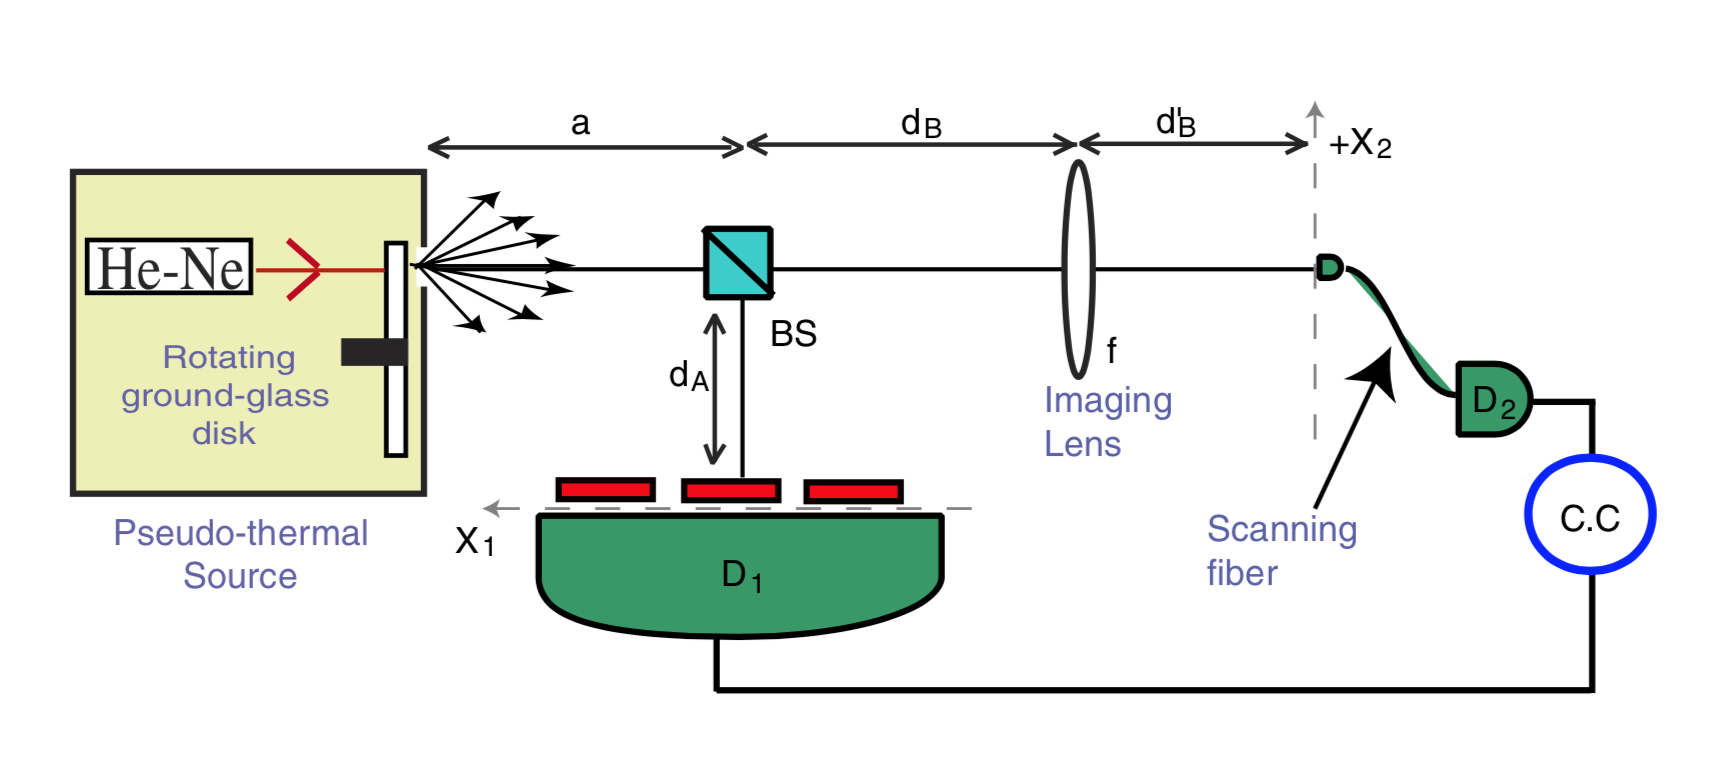
\includegraphics[width=0.6\textwidth]{Figures/thermalSetup.png}
\caption{Experimental setup for the Two-photon imaging using thermal light} 
\label{fig:thermalSetup}
\end{figure}
The source light in Figure \ref{fig:thermalSetup} is the one developed by Martinssen and Spiller\cite{intensity}
which is the most commonly used among the pseudothermal fields.
A  coherent laser radiation is focused on a rotating ground glass disk, 
the scattered radiation is chaotic with a Gaussian spectrum.




It is possible to establish an analogy
between classical optics and entangled two-photon optics:
the two-photon probability amplitude plays in entangled
two-photon processes the same role that the complex amplitude
of the electric field plays in classical optics  \cite{thermalAlejandra}.

\subsection{Computational Two-photon Imaging}

When we see the the different setups shown here, (Figures \ref{fig:twoPhotonSetup}, \ref{fig:pittman} and \ref{fig:thermalSetup}),
it can be noted that the transmitted path of the light, consists of a light beam propagating through air. What diferences these setup is the nature of the light used.
Specially in the setup using thermal light, the transmitted path is a classical phenomenon that can be simulated by a computer using Fresnel's propagation theory.
In Figure \ref{computationalSetup} we can see the setup for a Computational
Two-photon Imaging, where the transmitted path of the light is replaced by a computational simulation generated by a computer.
%image

The Computational Two-photon Imaging allows us to simulate the electric field data to be obtained before, during or after the data from the reflected arm is generated,
eliminating the need for collecting the data generated in the transmitted path. Also we have to use less opto-electronical elements on the optical table, simplifying 
the original setup and reducing considerably the amount of data generated. The resulting detection module consist only in one detector, a bucket detector that collects
 a single pixel (no spatial information) on light which has been transmitted through or reflected from the object.
In this situation only one light beam and one photodetector are required, this means that this imaging configuration cannot depend
on non-local two-photon interference.

Event though this realisation of the Two-photon Imaging is relevant in this discussion, 
because it is posible to retrive the image by precomputing the intensity fluctuation pattern that 
would have been seen by a high-spatial-resolution detector in a lensless two-photon imaging. 
It means we introduced some kind of coherence in this single path two-photon imaging. This is done by putting a CW
laser beam through a spatial light modulator (SLM) whose inputs are chosen to create the desired coherence behavior\cite{computational}.
A SLM is a special device that can manipulate light by modulating the amplitude, phase or polarization of the light waves in the two dimensions of space and time.
%----------------------------------------------------------------------------------------
%	SECTION 2
%----------------------------------------------------------------------------------------



